\documentclass[tikz,border=12pt]{standalone}
\usepackage[T1]{fontenc}
\usepackage{mathpazo}
\usepackage{amsmath,amssymb}
\usepackage{pifont}
\usetikzlibrary{arrows.meta, calc}

\definecolor{stblue}{HTML}{7B97AD}
\definecolor{rwgold}{HTML}{B8995E}
\definecolor{sage}{HTML}{7A9A7E}
\definecolor{dkbrown}{HTML}{3D3530}
\definecolor{wmgray}{HTML}{7B7067}
\definecolor{cream}{HTML}{F9F6F0}
\definecolor{border}{HTML}{D4C9B8}
\definecolor{terracotta}{HTML}{C47A6A}
\definecolor{lavender}{HTML}{907EA0}

\begin{document}
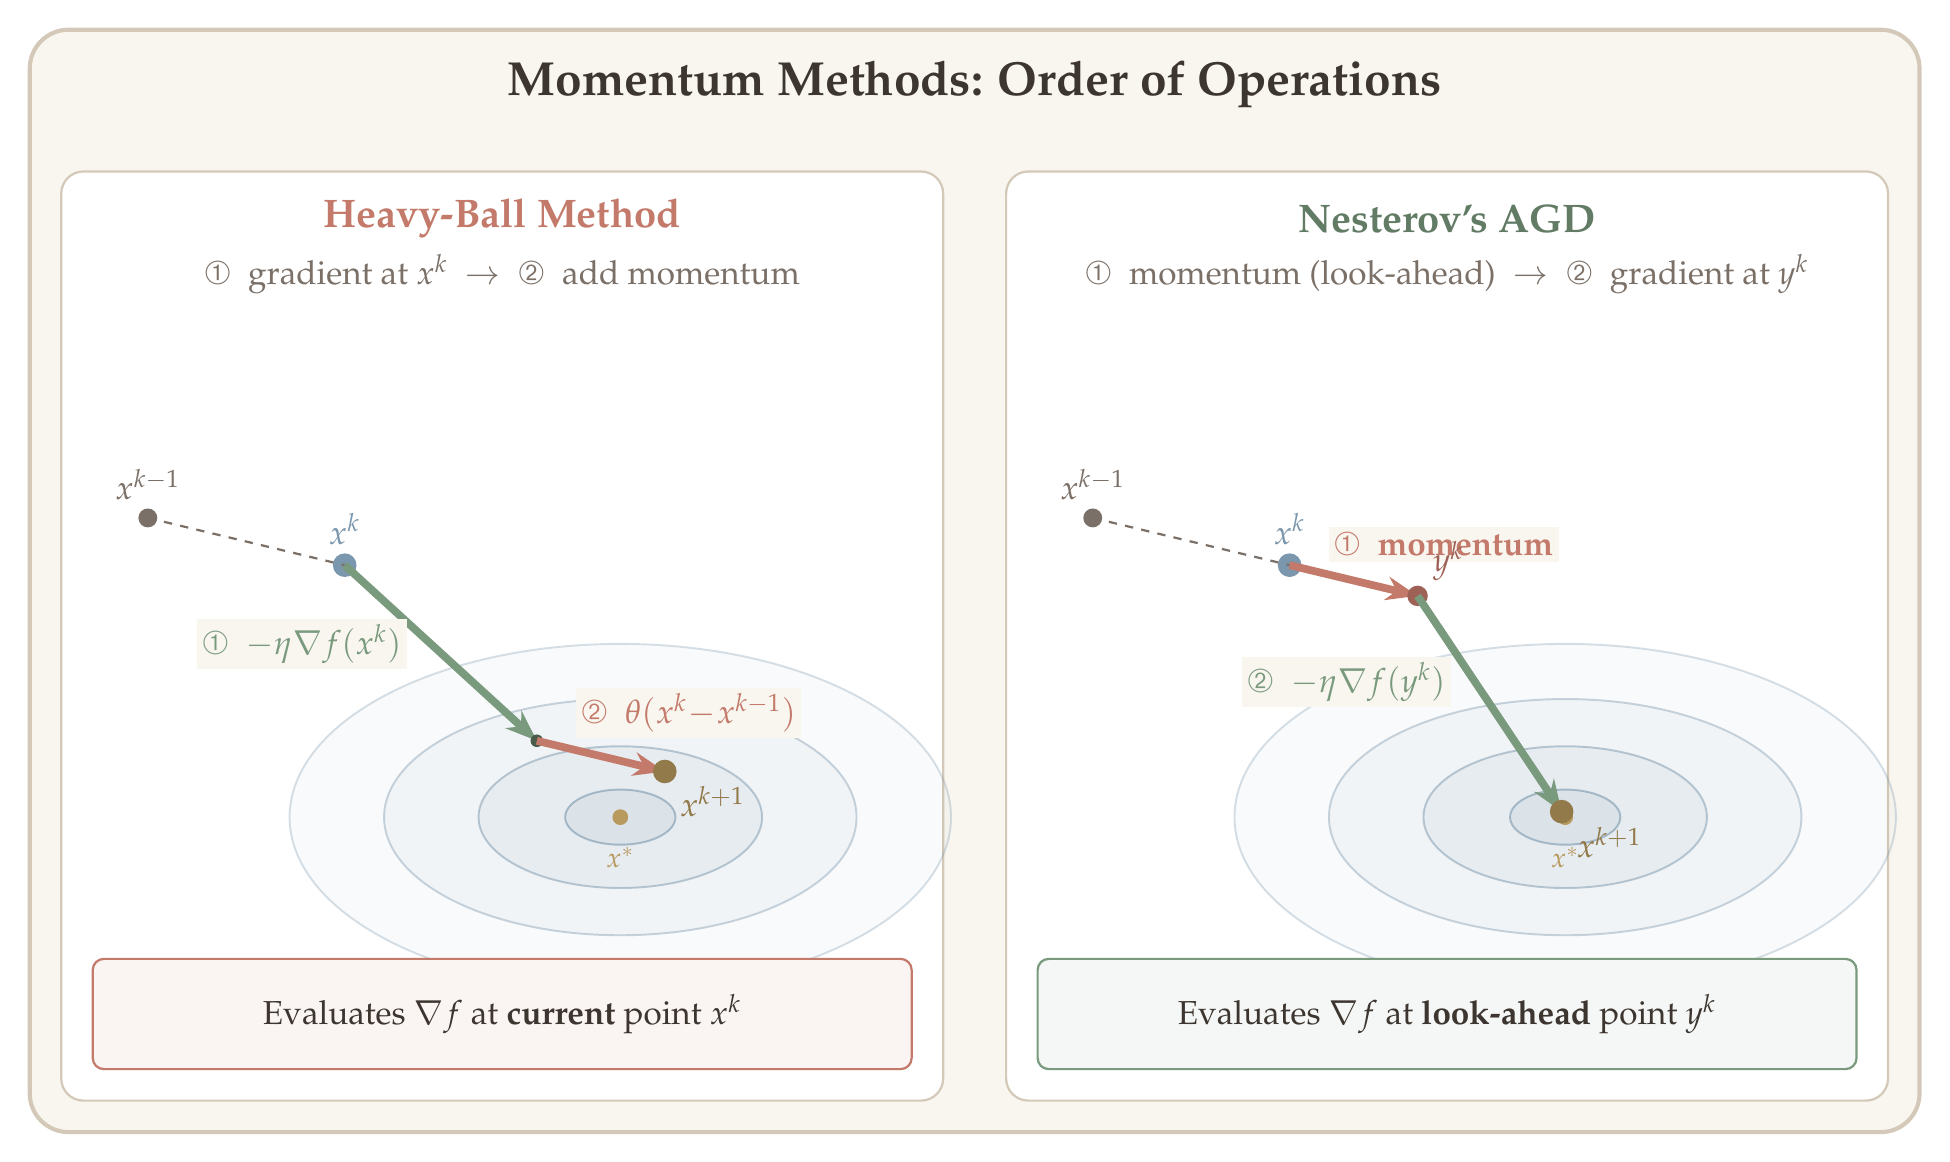
\begin{tikzpicture}[
  >={Stealth[length=4mm, width=3mm]},
  every node/.style={text=dkbrown, font=\large},
]

% Background
\fill[cream, rounded corners=14pt] (0,0) rectangle (24,14);
\draw[border, line width=1.5pt, rounded corners=14pt] (0,0) rectangle (24,14);

% Title
\node[font=\LARGE\bfseries, text=dkbrown] at (12,13.3)
  {Momentum Methods: Order of Operations};

% ============================================================
% LEFT PANEL: Heavy-Ball
% ============================================================
\fill[white, rounded corners=8pt] (0.4,0.4) rectangle (11.6,12.2);
\draw[border, line width=0.8pt, rounded corners=8pt] (0.4,0.4) rectangle (11.6,12.2);

\node[font=\Large\bfseries, text=terracotta] at (6,11.6) {Heavy-Ball Method};
\node[font=\large, text=wmgray] at (6,10.9)
  {\ding{192}\; gradient at $x^k$ \;$\to$\; \ding{193}\; add momentum};

% Contour ellipses — center at (7.5, 4.0), elongated horizontally
\fill[stblue, opacity=0.04] (7.5,4.0) ellipse (4.2 and 2.2);
\draw[stblue, line width=0.7pt, opacity=0.30] (7.5,4.0) ellipse (4.2 and 2.2);
\fill[stblue, opacity=0.06] (7.5,4.0) ellipse (3.0 and 1.5);
\draw[stblue, line width=0.7pt, opacity=0.40] (7.5,4.0) ellipse (3.0 and 1.5);
\fill[stblue, opacity=0.08] (7.5,4.0) ellipse (1.8 and 0.9);
\draw[stblue, line width=0.7pt, opacity=0.50] (7.5,4.0) ellipse (1.8 and 0.9);
\fill[stblue, opacity=0.10] (7.5,4.0) ellipse (0.7 and 0.35);
\draw[stblue, line width=0.7pt, opacity=0.60] (7.5,4.0) ellipse (0.7 and 0.35);

% Optimum
\fill[rwgold] (7.5,4.0) circle (0.1);
\node[font=\normalsize, text=rwgold, below=3pt] at (7.5,3.85) {$x^*$};

% ---- Points ----
% x^{k-1}
\coordinate (Lprev) at (1.5,7.8);
\fill[wmgray] (Lprev) circle (0.12);
\node[font=\large, text=wmgray, above=3pt] at (Lprev) {$x^{k-1}$};

% x^k  (direction from prev: (2.5, -0.6) — nearly horizontal)
\coordinate (Lk) at (4.0,7.2);
\fill[stblue] (Lk) circle (0.15);
\node[font=\large\bfseries, text=stblue, above=4pt] at (Lk) {$x^k$};

% Dashed trail: x^{k-1} -> x^k
\draw[wmgray, line width=0.8pt, dashed] (Lprev) -- (Lk);

% ---- Step 1: Gradient at x^k (sage) ----
% Direction toward optimum (7.5, 4.0): displacement (3.5, -3.2)
% |d| = 4.74, normalize to 3.3: scale = 0.696
% Displacement: (2.44, -2.23)
\coordinate (Lmid) at (6.44,4.97);
\draw[sage, line width=2.8pt, ->] (Lk) -- (Lmid);

% Label
\node[font=\large\bfseries, text=sage, fill=cream, inner sep=2pt, anchor=east]
  at ($(Lk)!0.45!(Lmid) + (-0.3,0.0)$)
  {\ding{192}\; $-\eta\nabla f(x^k)$};

% Small dot at intermediate
\fill[sage!60!black] (Lmid) circle (0.08);

% ---- Step 2: Momentum from intermediate (terracotta) ----
% Direction = x^k - x^{k-1} = (2.5, -0.6), scale theta=0.65: (1.625, -0.39)
\coordinate (Lnext) at ($(Lmid) + (1.625,-0.39)$);
\draw[terracotta, line width=2.8pt, ->] (Lmid) -- (Lnext);

% Label
\node[font=\large\bfseries, text=terracotta, fill=cream, inner sep=2pt, anchor=south west]
  at ($(Lmid)!0.3!(Lnext) + (0.0,0.15)$)
  {\ding{193}\; $\theta(x^k\!-\!x^{k-1})$};

% x^{k+1}
\fill[rwgold!80!black] (Lnext) circle (0.15);
\node[font=\large\bfseries, text=rwgold!80!black, below right=2pt] at (Lnext)
  {$x^{k+1}$};

% ---- Bottom key-point box ----
\fill[terracotta!8, rounded corners=4pt] (0.8,0.8) rectangle (11.2,2.2);
\draw[terracotta, line width=0.8pt, rounded corners=4pt] (0.8,0.8) rectangle (11.2,2.2);
\node[font=\large, text=dkbrown, align=center] at (6.0,1.5)
  {Evaluates $\nabla f$ at \textbf{current} point $x^k$};

% ============================================================
% RIGHT PANEL: Nesterov's AGD
% ============================================================
\fill[white, rounded corners=8pt] (12.4,0.4) rectangle (23.6,12.2);
\draw[border, line width=0.8pt, rounded corners=8pt] (12.4,0.4) rectangle (23.6,12.2);

\node[font=\Large\bfseries, text=sage!80!black] at (18,11.6) {Nesterov's AGD};
\node[font=\large, text=wmgray] at (18,10.9)
  {\ding{192}\; momentum (look-ahead) \;$\to$\; \ding{193}\; gradient at $y^k$};

% Contour ellipses — center at (19.5, 4.0), same shape
\fill[stblue, opacity=0.04] (19.5,4.0) ellipse (4.2 and 2.2);
\draw[stblue, line width=0.7pt, opacity=0.30] (19.5,4.0) ellipse (4.2 and 2.2);
\fill[stblue, opacity=0.06] (19.5,4.0) ellipse (3.0 and 1.5);
\draw[stblue, line width=0.7pt, opacity=0.40] (19.5,4.0) ellipse (3.0 and 1.5);
\fill[stblue, opacity=0.08] (19.5,4.0) ellipse (1.8 and 0.9);
\draw[stblue, line width=0.7pt, opacity=0.50] (19.5,4.0) ellipse (1.8 and 0.9);
\fill[stblue, opacity=0.10] (19.5,4.0) ellipse (0.7 and 0.35);
\draw[stblue, line width=0.7pt, opacity=0.60] (19.5,4.0) ellipse (0.7 and 0.35);

% Optimum
\fill[rwgold] (19.5,4.0) circle (0.1);
\node[font=\normalsize, text=rwgold, below=3pt] at (19.5,3.85) {$x^*$};

% ---- Points (same relative positions) ----
% x^{k-1}
\coordinate (Rprev) at (13.5,7.8);
\fill[wmgray] (Rprev) circle (0.12);
\node[font=\large, text=wmgray, above=3pt] at (Rprev) {$x^{k-1}$};

% x^k
\coordinate (Rk) at (16.0,7.2);
\fill[stblue] (Rk) circle (0.15);
\node[font=\large\bfseries, text=stblue, above=4pt] at (Rk) {$x^k$};

% Dashed trail: x^{k-1} -> x^k
\draw[wmgray, line width=0.8pt, dashed] (Rprev) -- (Rk);

% ---- Step 1: Momentum / look-ahead (terracotta) ----
% Same momentum vector: 0.65*(2.5, -0.6) = (1.625, -0.39)
\coordinate (Ryk) at ($(Rk) + (1.625,-0.39)$);  % y^k = (17.625, 6.81)
\draw[terracotta, line width=2.8pt, ->] (Rk) -- (Ryk);

% Label
\node[font=\large\bfseries, text=terracotta, fill=cream, inner sep=2pt, anchor=south west]
  at ($(Rk)!0.3!(Ryk) + (0.0,0.15)$)
  {\ding{192}\; momentum};

% y^k point
\fill[terracotta!80!black] (Ryk) circle (0.13);
\node[font=\large\bfseries, text=terracotta!80!black, above right=2pt] at (Ryk)
  {$y^k$};

% ---- Step 2: Gradient at y^k (sage) ----
% Direction from y^k toward optimum (19.5, 4.0): (1.875, -2.81)
% |d| = 3.38, normalize to 3.3: scale = 0.976
% Displacement: (1.83, -2.74)
\coordinate (Rnext) at ($(Ryk) + (1.83,-2.74)$);  % ≈ (19.46, 4.07)
\draw[sage, line width=2.8pt, ->] (Ryk) -- (Rnext);

% Label
\node[font=\large\bfseries, text=sage, fill=cream, inner sep=2pt, anchor=east]
  at ($(Ryk)!0.4!(Rnext) + (-0.3,0.0)$)
  {\ding{193}\; $-\eta\nabla f(y^k)$};

% x^{k+1}
\fill[rwgold!80!black] (Rnext) circle (0.15);
\node[font=\large\bfseries, text=rwgold!80!black, below right=2pt] at (Rnext)
  {$x^{k+1}$};

% ---- Bottom key-point box ----
\fill[sage!8, rounded corners=4pt] (12.8,0.8) rectangle (23.2,2.2);
\draw[sage, line width=0.8pt, rounded corners=4pt] (12.8,0.8) rectangle (23.2,2.2);
\node[font=\large, text=dkbrown, align=center] at (18.0,1.5)
  {Evaluates $\nabla f$ at \textbf{look-ahead} point $y^k$};

\end{tikzpicture}
\end{document}
